\begin{figure}
\fbox{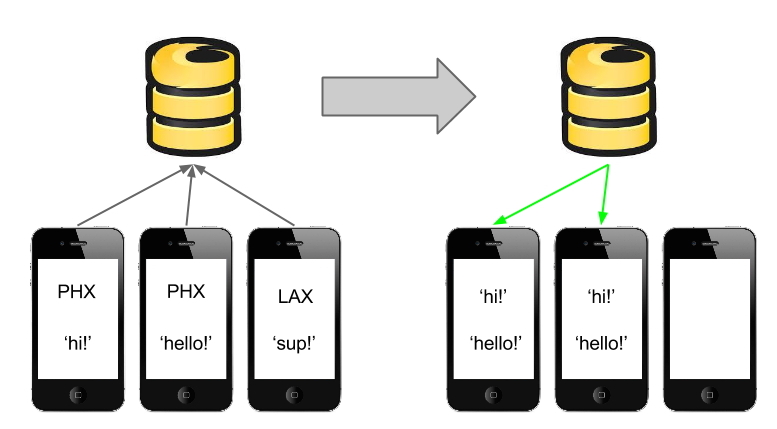
\includegraphics[width=.48\textwidth]{figs/chatExample}}
\caption{Chat example for local chat.  When users are chatting in local mode they will not see messages from users that are far away.  For example two users that are nearby in Phoenix will see messages from one another, while a user in Los Angeles will not see those messages.}
\label{chatExample}
\end{figure}

\subsection{Client Side(iOS application)}
In order to keep track of users and their locations we implemented a login system and location services.  The application is set to upload the users location to the server at set time intervals (10 minutes by default), to be used for determining to which zones a user belongs.  The iOS application acts primarily as a tracking beacon and data conduit for the user.  The phone performs minimal computation, both because it is not a trusted asset within the system, and also because computations would adversely influence the battery life of the device.  Upon login in users are presented with a zones that they are associated with, where a zone is their current location or one of their previous locations.  After selecting a zone the user is presented with a message thread that allows them to post messages, receive new updates, and read older posts. When a user makes a new post their message is automatically tagged with additional metadata: geolocation of the post, the zone it was posted to, timestamp, and the user that posted it. When users post based on their current location the message will be shown to other users that are nearby as in Figure~\ref{chatExample}.  Users can also post their updates to a zone that they are associated with, which doesn't necessarily require them to be in the same geographic location.  Those messages are passed along as in Figure~\ref{zones}

\begin{figure}
\fbox{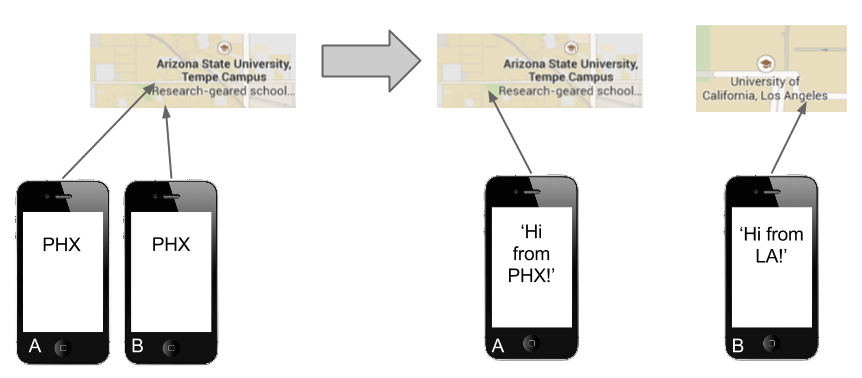
\includegraphics[width=.48\textwidth]{figs/zones}}
\caption{Chat example with zones.  When users are chatting in zones mode they will be able to chat in a zone even if they are not currently located in that zone. So for example if 2 users were present at ASU and afterwards one user went to UCLA  (or anywhere) they would still be able to communicate for a few days, because of their previous association with ASU.  }
\label{zones}
\end{figure}

\subsection{Server Side(Cloud Code \& Firebase)}
% Christophe, can you add more to what I have and maybe change so it doesn't sounds like we just copied and paste?
% URL for reference if needed, http://jormungand.net/projects/misc/em/
Most heavy lifting occurs on the server side where we have less limitations on resources.  In particular Parse allows processing in 15-second chunks on their high-performance distributed computing system, running a form of Javascript.  This means that if tasks can be parallelized easily they can run free, and also very very quickly.  As a result we discovered a Javascript implementation of the Expectation Maximization(EM) algorithm and modified it to work within the confines of Parse Cloud Code.  To handle the data flow we first pull all the user data down from Firebase, the users are returned as JSON objects. The user information is then stripped down to a time-series of locations, which are then separated and treated as a single time point. The location data is then passed into the EM algorithm to calculate clusters and user-cluster relationship.  Once the clusters are calculated the Google Places API is invoked to name the zones.  In practice We had significant difficulties getting intelligible results from Google Places API, ``ASU" became ``ASU Undergraduate Admissions" or ``ASU Museum", so zone names were manually curated.   It looks like the Google Places API would be appropriate to use when dealing with small zones, like a museum or stadium for a football game.  Or perhaps for very large zones such as "Tempe", but it seems to have significant difficulties when naming mid-sized zones.  After the zones are created they are pushed back into Firebase so that they can be accessed by users.  One implementation limitation is the transition of messages between zones.  When the zones are recreated it is probable that most zones will be fairly static (e.g. a generic ASU zone should be maintained),  so we should be able to create a measure of difference between gaussians (mean and covariance matrixes) to automatically reassign messages from relocated zones.  Similarly we don't currently allow for changes in the number of zones, which means that for a new zone to appear it needs to not only be strong enough to form, but it must also be a tighter zone than another currently existing zone.  This limitation could be overcome fairly easily by measuring a gradient-descent of the error as we add more zones to the clustering as described in~\cite{ray1999determination}.







 